% \documentclass[11pt]{aghdpl}
\documentclass[en,11pt]{aghdpl}  % praca w języku angielskim

% Lista wszystkich języków stanowiących języki pozycji bibliograficznych użytych w pracy.
% (Zgodnie z zasadami tworzenia bibliografii każda pozycja powinna zostać utworzona zgodnie z zasadami języka, w którym dana publikacja została napisana.)
\usepackage[english]{babel}

% Użyj polskiego łamania wyrazów (zamiast domyślnego angielskiego).
% \usepackage{polski}

\usepackage[utf8]{inputenc}

% dodatkowe pakiety

% \usepackage{geometry}
\usepackage{mathtools}
\usepackage{amsfonts}
\usepackage{amsmath}
\usepackage{amsthm}

\usepackage{float}

% --- < bibliografia > ---

% \usepackage[
% style=numeric,
% sorting=none,
% %
% % Zastosuj styl wpisu bibliograficznego właściwy językowi publikacji.
% language=english,
% % autolang=other,
% % Zapisuj datę dostępu do strony WWW w formacie RRRR-MM-DD.
% urldate=iso8601,
% % Nie dodawaj numerów stron, na których występuje cytowanie.
% backref=false,
% % Podawaj ISBN.
% isbn=false,
% url=true,
% %
% % Ustawienia związane z polskimi normami dla bibliografii.
% maxbibnames=3,
% % Jeżeli używamy BibTeXa:
% backend=bibtex
% ]{biblatex}

\usepackage[
    style=numeric,
    backend=bibtex
]{biblatex}

% \usepackage{csquotes}
% Ponieważ `csquotes` nie posiada polskiego stylu, można skorzystać z mocno zbliżonego stylu chorwackiego.
% \DeclareQuoteAlias{croatian}{polish}

\addbibresource{bibliografia.bib}

% Nie wyświetlaj wybranych pól.
%\AtEveryBibitem{\clearfield{note}}


% ------------------------
% --- < listingi > ---

% Użyj czcionki kroju Courier.
\usepackage{courier}

\usepackage{listings}
\lstloadlanguages{TeX}

\lstset{
  literate={ą}{{\k{a}}}1
           {ć}{{\'c}}1
           {ę}{{\k{e}}}1
           {ó}{{\'o}}1
           {ń}{{\'n}}1
           {ł}{{\l{}}}1
           {ś}{{\'s}}1
           {ź}{{\'z}}1
           {ż}{{\.z}}1
           {Ą}{{\k{A}}}1
           {Ć}{{\'C}}1
           {Ę}{{\k{E}}}1
           {Ó}{{\'O}}1
           {Ń}{{\'N}}1
           {Ł}{{\L{}}}1
           {Ś}{{\'S}}1
           {Ź}{{\'Z}}1
           {Ż}{{\.Z}}1,
  basicstyle=\footnotesize\ttfamily,
}

% ------------------------

\AtBeginDocument{
  \renewcommand{\tablename}{Table}
  \renewcommand{\figurename}{Figure}
}

% ------------------------
% --- < tabele > ---

\usepackage{array}
\usepackage{tabularx}
\usepackage{multirow}
\usepackage{booktabs}
\usepackage{makecell}
\usepackage{blindtext}
\usepackage[flushleft]{threeparttable}

% defines the X column to use m (\parbox[c]) instead of p (`parbox[t]`)
\newcolumntype{C}[1]{>{\hsize=#1\hsize\centering\arraybackslash}X}


%---------------------------------------------------------------------------

\author{Dariusz Czajkowski, Grzegorz Tłuszcz}
\shortauthor{D. Czajkowski, G. Tłuszcz}

%\titlePL{Przygotowanie bardzo długiej i pasjonującej pracy dyplomowej w~systemie~\LaTeX}
%\titleEN{Preparation of a very long and fascinating bachelor or master thesis in \LaTeX}

\titlePL{}
\titleEN{Modeling movement of people using a mobile application}


\shorttitlePL{}
\shorttitleEN{Modeling movement of people using a mobile application}

\thesistype{Modeling and Simulation of Systems}
%\thesistype{Master of Science Thesis}

\supervisor{dr hab. inż. Jarosław Wąs}
% \supervisor{Jarosław Wąs PhD, DSc}

% \degreeprogramme{Informatyka}
\degreeprogramme{Computer Science}

\date{2018}

% \department{Katedra Informatyki Stosowanej}
\department{}

% \faculty{Wydział Elektrotechniki, Automatyki,\protect\\[-1mm] Informatyki i Inżynierii Biomedycznej}
\faculty{Faculty of Electrical Engineering, Automatics, Computer Science and Biomedical Engineering}

\acknowledgements{}


\setlength{\cftsecnumwidth}{10mm}

%---------------------------------------------------------------------------
\setcounter{secnumdepth}{4}
\brokenpenalty=10000\relax

\begin{document}

\titlepages

% Ponowne zdefiniowanie stylu `plain`, aby usunąć numer strony z pierwszej strony spisu treści i poszczególnych rozdziałów.
\fancypagestyle{plain}
{
  % Usuń nagłówek i stopkę
  \fancyhf{}
  % % Usuń linie.
  \renewcommand{\headrulewidth}{0pt}
  \renewcommand{\footrulewidth}{0pt}
  % \fancyhf{}
  % \fancyhead{}
  %\fancyhead[L]{\slshape{\small \rightmark}}
  % \fancyhead[L]{\slshape{\small \rightmark}}
  % \fancyhead[RO,LE]{\slshape{\small \rightmark}}
  %\fancyhead[R]{\bfseries \thepage}
  % \fancyhead[R]{\bfseries \thepage}
}

\renewcommand{\contentsname}{Table of Contents}
\renewcommand{\bibname}{References}
\setcounter{tocdepth}{2}
\tableofcontents
\clearpage

\chapter{Introduction}

\blindtext[6]

\chapter{Literature review}

In this chapter, we would like to focus on existing approaches to GPS data collection and postprocessing. Our goal is also to learn about possible ways of data filtering, travel modes detection and route approximation.

According to many of the reviewed publications, locations can be acquired using one of many technologies e.g. Geographic Information Systems (GIS), Radio Frequency Identification (RFID), Wireless Local Area Network (WLAN) and Global Positioning System (GPS). It is worth mentioning that the latter is by far the most popular and easiest to implement on a large scale. This is because such locations can be obtained using a module built into smartphones so there is no need for an additional device. Except for geolocalization data, engineers also collect acceleration, direction and height above the sea level. A popular solution is to use a mobile app for localization sampling and displaying results. Obtaining essential data can be performed in some interval (eg. 10 seconds) or after parameters' change. This allows them to achieve regular, accurate data in terms of time or location.

After collecting GPS samples many of the authors mention some way of data filtering to reduce further complications in computation. One of the problems with GPS is that the signal weakens inside buildings and dense livelihood. In other words, the points appearing to be falling inside a building may or may not be actually taken indoor, and vice versa. This is because signals are attenuated, reflected and scattered by roofs, walls and other objects. To solve this issue Yongyao Jiang in his work "Automated Human Mobility Mode Detection Based on GPS Tracking Data" used building footprints obtained from the state Massachusetts Office of Geographic Information (MassGIS) overlaid with given GPS points.  Another interesting difficulty is to determine the travelling mode of the user. One of the approaches is to measure average speed and determine some threshold values to distinguish walking, riding a bike and travelling by car.

A man can perform data clustering based on travelling mode to remove undesired activities.  Another interesting solution is to use the accelerometer combined with time measurements to decide if any steps were made during the tour. That way they can determine which travels were made with a vehicle. Some of the engineers behind the publications even reached for machine learning algorithms to recognize walking habits and to label them as 'walking activity'.

\begin{figure}[]
    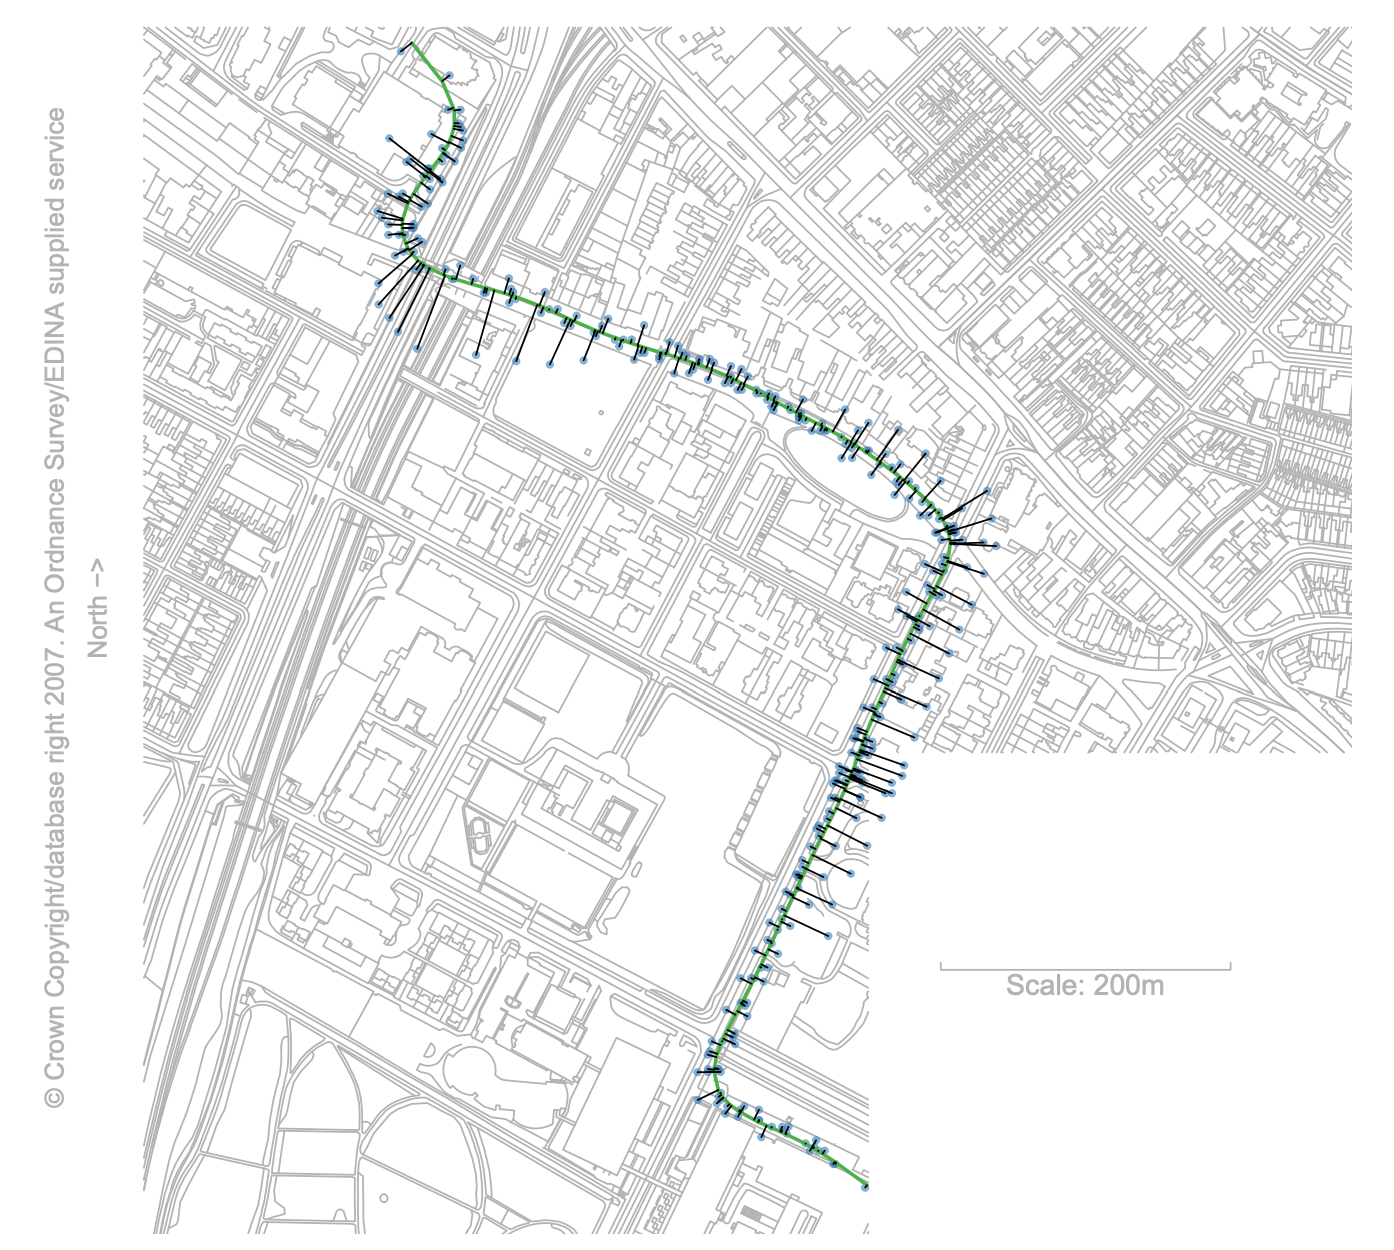
\includegraphics[width=0.8\textwidth]{images/article-map.png}
    \caption{Robust principal curve (green) fitted to GPS point cloud data. \\ \textit{source: Chris Brunsdon, Path Estimation from GPS Tracks}}
    \label{fig:chrismap}
\end{figure}

Last but not least, authors face a problem with displaying results. Algorithms often return discrete data (points) with various accuracy. It is important to somehow approximate walked path on the map. This task can be achieved using principal curves created from locations grouped into a singular path. Chris Brunsdon in his work\cite{cb} gives a good example of the algorithm for computing such a curve \ref{fig:chrismap}. Einbeck, Tutz and Evers in their work\cite{ete} dive deep into the process of constructing these curves and the benefits from choosing various methods.

\chapter{Proposed model of the phenomenon} \label{ch:model}

\section{The model's purpose and description}
Our goal is to build a mobile application that would allow users to review their past walking paths and the current position of their friends. The majority of the effort is focused on implementing a backend API that would filter out corrupted samples and create paths representing routes walked by the user in the past. Frontend mobile application retrieves data from the API and displays it on the map. It also handles all the user interactions and sends current user location.

\section{Algorithm assumptions}
Our algorithm assumes that:
\begin{enumerate}
    \item mobile application is turned on forever,
    \item mobile phones send requests with their location every 5 seconds,
    \item user tracks only outdoor activities,
    \item user cannot walk faster than 14 km/h.
    \item movement with average speed higher than 14 km/h is considered as travel with a vehicle.
\end{enumerate}

Due to the fact that we have limited deployment possibilities, we launched our app with Expo and it is only able to retrieve GPS location when the app is turned on.

\section{Activity cycle diagrams}

\subsection{Front-end app cycle}
The \ref{fig:front} shows the front-end app cycle diagram. The app is very simple in its flow. It simply gets the GPS signal and sends it to the API every 5 seconds. The app also has two modes. One of them allows to see current position of all the users. The second mode displays a history of a specific user.

\begin{figure}[p]
    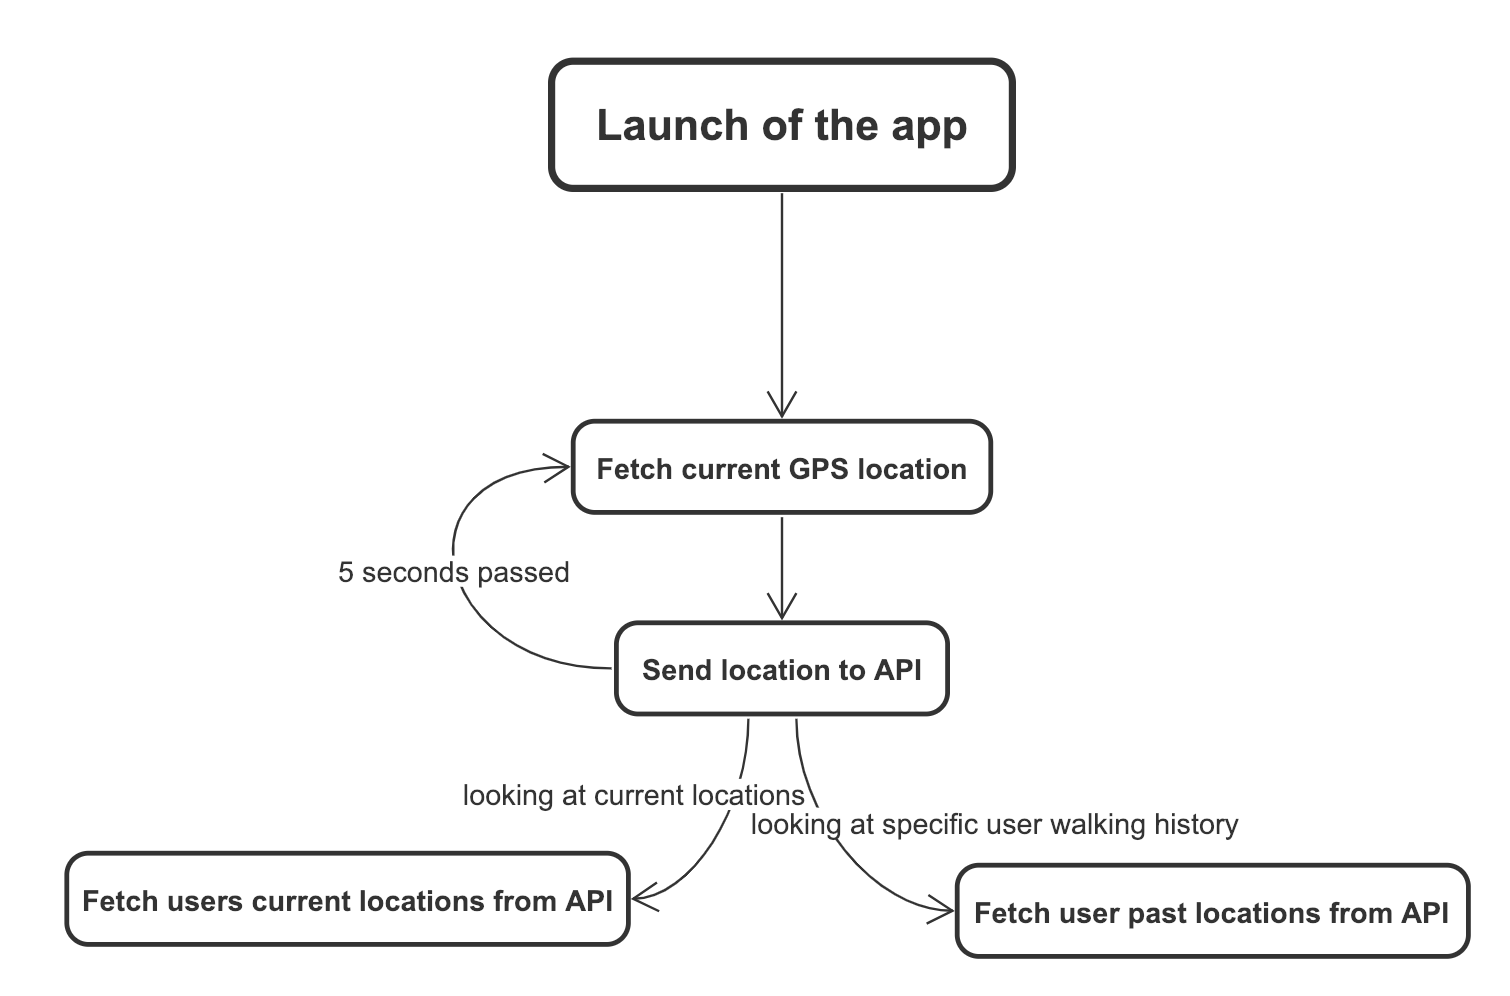
\includegraphics[width=0.9\textwidth]{images/front.png}
    \caption{Front-end app cycle \\ \textit{source: own elaboration}}
    \label{fig:front}
\end{figure}

\subsection{Sending current location to the API}
When the app sends the location along with user's id to the API, the API has to do some calculations depicted in \ref{fig:api} to validate provided data.

\begin{figure}[H]
    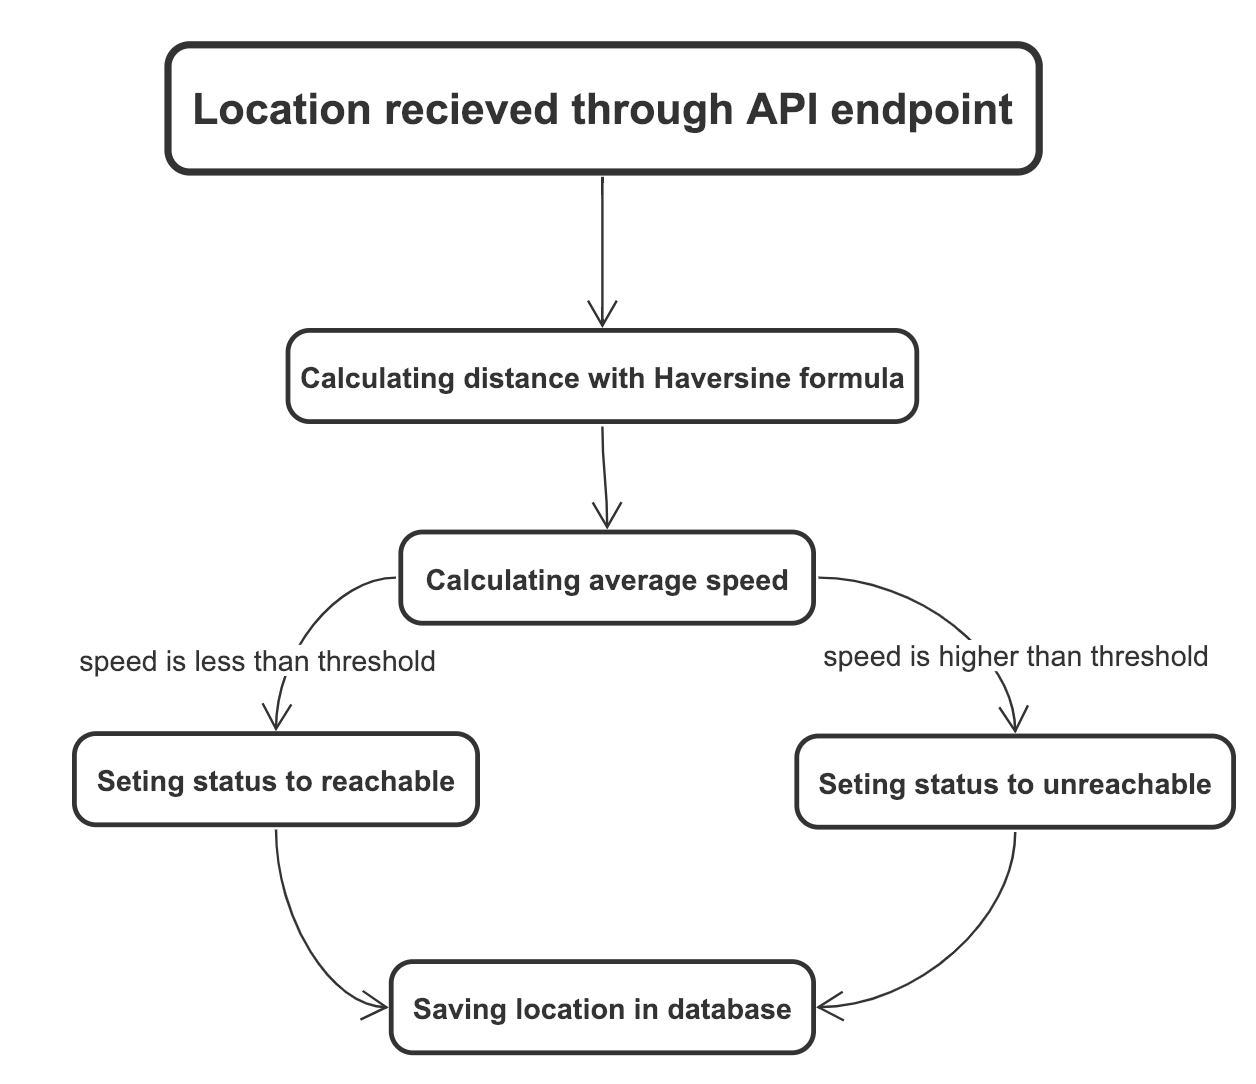
\includegraphics[width=0.9\textwidth]{images/api.png}
    \caption{Sending current location to the API \\ \textit{source: own elaboration}}
    \label{fig:api}
\end{figure}

\subsection{Fetching historical locations}
When the app asks for historical locations, the API calculates on-the-fly if points are reachable and removes all invalid data. This is done every time the app asks for locations to allow tweaking of the algorithm at any moment. If these calculations became expensive, everything could be cached and the cache would be invalidated whenever a new version of the algorithm arrives. The flow can be seen in \ref{fig:history}.

\begin{figure}[p]
    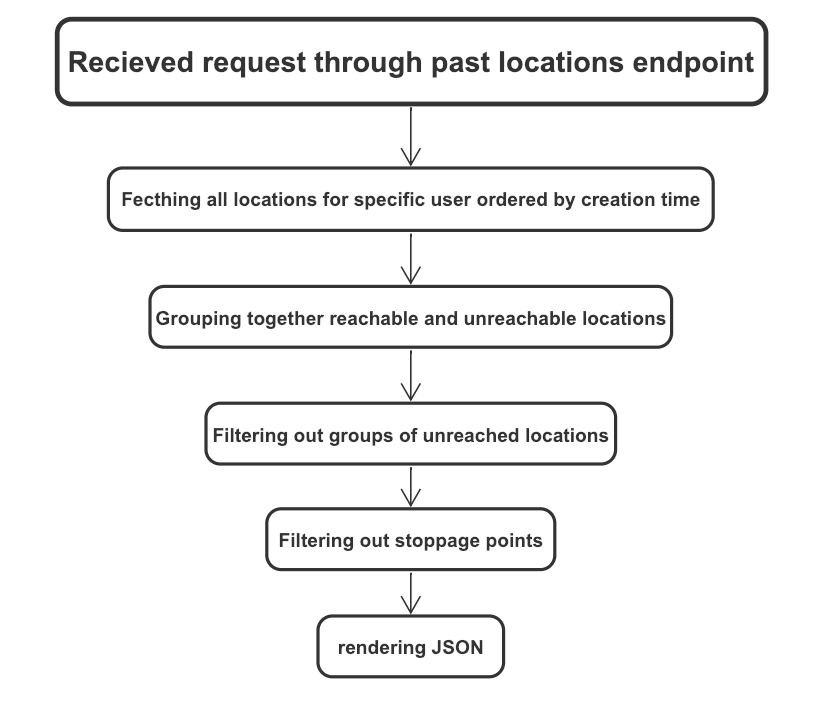
\includegraphics[width=0.9\textwidth]{images/history.png}
    \caption{Fetching historical locations \\ \textit{source: own elaboration}}
    \label{fig:history}
\end{figure}

\section{Applied approach compared to other implementations}

As well as many other engineers we collected locations using GPS technology. In our approach, we used three key components to reach our goal. First of them is calculating the average speed of the user based on his last location and current position. To achieve that we used Haversine formula which is quite unique considering other implementations. Then we experimentally stated some threshold values which were taking into consideration GPS errors. Based on the final judgment we set the status of the location either as reachable or unreachable.

The second one is an algorithm that filters out unreachable locations. In other words, it filters out travelling modes other than walking. This idea is widely known and we thought that it fits our needs.

The third one is a piece of code which aims to remove stoppage points, mainly occurred by traffic light stops and staying in traffic jams. It is our own idea and differs from other projects.

\section{The use case diagram}

\begin{figure}[H]
    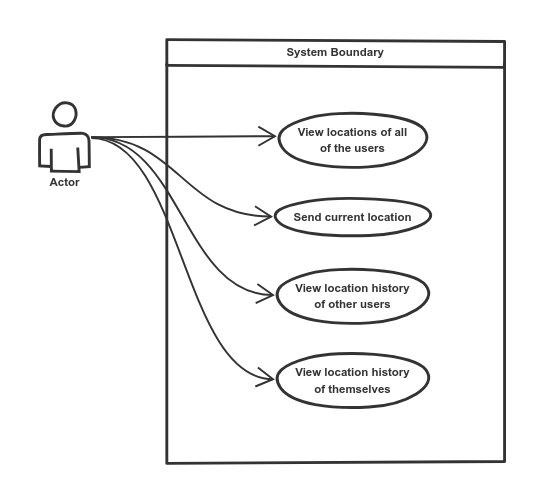
\includegraphics[width=0.9\textwidth]{images/diagram.png}
    \caption{The use case diagram \\ \textit{source: own elaboration}}
\end{figure}

\chapter{Simulation of the phenomenon - implementation}

\section{Technology and tools}

The project described in this work is written in two parts --- backend and the app.

As we could pick any technology whatsoever we picked Ruby for the backend as this is the backend technology we are most familiar with. We have also picked a web framework called Ruby on Rails as it is the most popular web framework for Ruby. In the long run, it saved us a lot of time that would be required to set up a web server, handle requests, make database queries and many more.

The backend consists of a few REST\footnote{Representational State Transfer} endpoints. One of them receives user's location and runs the algorithm against provided location to determine, whether the input is legitimate or not. After it is calculated, data is preserved in a database with an appropriate label. There is also an endpoint to list locations of all users at the time and an endpoint to return specific user's history.

Implementing a mobile application didn't seem like an easy task at first. Currently, if someone wants to make a mobile application they have to target a specific platform --- Android or iOS. Developing for these platforms isn't easy at all. For the Android development, you have to know Java, Kotlin or C++, have Android Studio installed, and knowledge on what to do. Fortunately, there are many resources on how to start. Authors of this work do not have an Android phone, so there would be issues with running the app in a simulator, which would defeat the purpose of this work. The iOS side of things is not easier either, as it requires knowledge of Swift or Objective-C, having XCode installed on a macOS device, a paid developer account and many more. Even if we decided to go with iOS, it would require a lot of work, time and resources to develop a simple app. At that point, we started reading through the Internet and we learned there are many JavaScript compilers that compile your code into native-to-the-platform code. One of them is React Native --- a technology that allows writing JavaScript code in a React Framework that is compiled to a native app. This made great news to us, as we didn't have to learn any other tools or languages, as we know JavaScript perfectly well.

The app consists of a view that presents a native-to-iOS map. On the map, there are markers that represent locations of all app users in real time. If a marker is held, more details about the location are shown --- a name of the user and the time of the measurement. When a marker is clicked, the map goes into the \textit{history} mode where all historical locations of that particular user are displayed. You can then click anywhere on the map to go back to the \textit{normal} mode. In the background, any time the app is open, current location of the user is sent to the server to update user's location.

\section{Implementation details}
In this section, we will describe two main algorithms used to store locations and retrieve past walking paths of the user.

In our database, we have two tables: one for representing users and one for locations. I will refer to the model of a user with \textit{User} and to a location with \textit{Location}.

The process of storing a new sample consists mainly of computing average speed needed to achieve new location. To compute the distance between to points we use Haversine formula which is described as below:

\begin{equation}
    \displaystyle d=2r\arcsin \left({\sqrt {\sin ^{2}\left({\frac {\varphi _{2}-\varphi _{1}}{2}}\right)+\cos(\varphi _{1})\cos(\varphi _{2})\sin ^{2}\left({\frac {\lambda _{2}-\lambda _{1}}{2}}\right)}}\right)
\end{equation}
where~$\varphi _{1},\varphi _{2}$~are~latitudes~and~$\lambda _{1},\lambda _{2}$~are~longitudes.

Here is some pseudo code of the storing algorithm:
\begin{lstlisting}
my_user = User.find(user_id)
last_location = my_user.locations().last()
distance = Haversine(new_location, last_location)
time = new_location.creation_time() - last_location.creation_time()
speed = distance / time
if (speed > threshold)
    new_location.status = unreachable
else
    new_location.status = reachable
end
return new_location.save()
\end{lstlisting}
Another crucial part of our system is the algorithm rendering old paths. Here you can get a quick glimpse of it:
\begin{lstlisting}
my_user = User.find(user_id)
my_user.locations()
routes = [] // group reachable locations into walking paths
counter = 0

for (location in locations)
    if (location.status == reachable)
        routes[counter].push(location)
    else
        if (routes[counter] != null)
            counter+=1
        end
    end
end

// remove stoppage points
routes.filter do (path)
    // calculating center of mass in path
    com = {lat: 0, lon: 0}

    for (location in path)
        com.lat += location.lat
        com.lon += location.lon
    end

    com.lat /= path.size()
    com.lon /= path.size()

    // check if there is a point in the path
    // further than a threshold from the centre of mass
    return path.any do (location)
        distance = Haversine(location, com)
        return distance > threshold
    end
end
\end{lstlisting}
As you can see we group reachable locations together and after grouping, we check if any of the paths in routes has all of its locations in a small area. This would mean that probably this path is actually a temporary stoppage on traffic lights and we do not want to render it as walking.

\chapter{Results of the simulation}
\section{Statistics and gathered results}

During the testing phase of the app we have gathered more than 8000 location records that had to be filtered and ran through our algorithm. We have made a total of 21 paths with walking, bus riding and car driving. During testing, we have tweaked the algorithm for it to show as accurate results, as possible. We think, the app performs alright, but the accuracy of the GPS signal could be improved.

\section{Algorithm calibration and data validation}

During the development phase we have picked 9 km/h as a maximum of human walking speed and set that as a limit. After making a few passes and trying the app out, we have found 9 km/h to be not enough, as it removes any kind of running and does not take into consideration GPS inaccuracy. What we have discovered, is that if someone moved 12 meters, which makes it a plausible distance to be walked in as depicted in the equation \ref{eq:distancespeed}, GPS inaccuracy made that distance to be 14 meters, which removed the readout.
\begin{equation} \label{eq:distancespeed}
    t = 5[s];~~ x = 12[m];~~ \bar{v} = \frac{\Delta x}{\Delta t} = \frac{12}{5} [\frac{m}{s}] = 2.4 [\frac{m}{s}] = 7.2 [\frac{km}{h}] < 9 [\frac{km}{h}]
\end{equation}
After some testing, we have found 20 km/h to be an optimal value. It does not exclude runners, but does correctly filter any car driving, as we have found a 30 km/h to be a minimum value a car moves in, even when going through speed bumps. The only exception is a standstill or a very slowly moving traffic jam. Our algorithm does filter out any standstill, but cannot handle a very slowly moving car. It would be invalid to assume someone is in a slowly moving car, as it is very possible they are walking at that moment. Perhaps a look at a larger picture, taking into consideration more context would help, but machine learning could be a valid solution as well.

\section{Comparison of the results with real data}

We have put a lot of time to validate data and polish the algorithm to give the best results possible. In the following subsections, there are a few examples presented. They should give the reader a whole picture on how the app works and what is happening behind the scenes.

\begin{figure}[]
    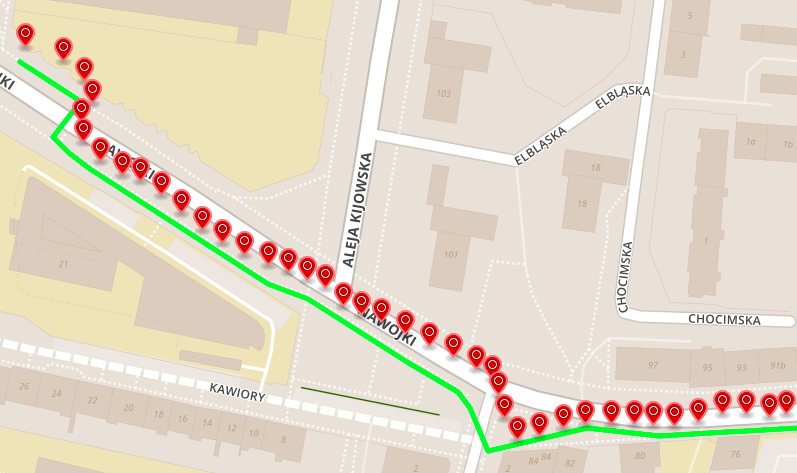
\includegraphics[width=0.9\textwidth]{images/1.png}
    \caption{Green path is the actual path, red pins depict non-filtered readouts. \\ \textit{source: own elaboration}}
    \label{fig:screenexample1}
\end{figure}

\subsection{Example 1: Accurate walking readouts}

This is an example, when readouts during walking are correctly read and displayed on the map. As can be seen in the figure \ref{fig:screenexample1}, presented location differs from actual position a little due to GPS inaccuracy. This inaccuracy is not substantial and is not a subject of this work.

\begin{figure}[]
    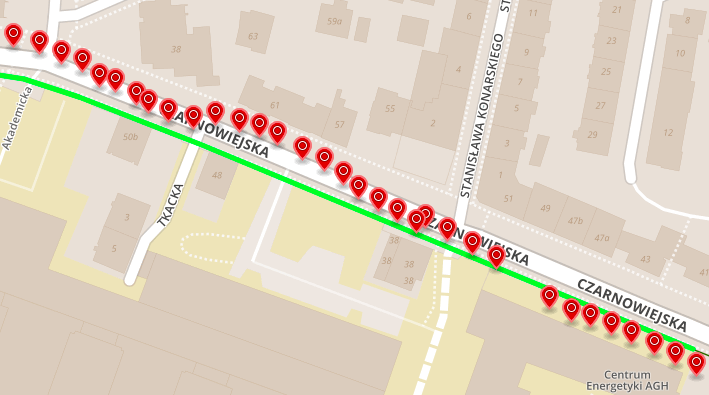
\includegraphics[width=0.9\textwidth]{images/1-1.png}
    \caption{Green path is the actual path, red pins depict non-filtered readouts. \\ \textit{source: own elaboration}}
    \label{fig:screenexample11}
\end{figure}

\begin{figure}[]
    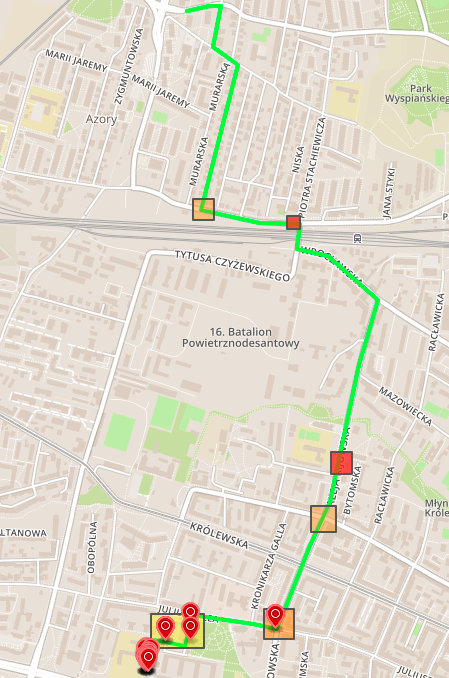
\includegraphics[width=0.9\textwidth]{images/2.png}
    \caption{Green path is the actual path, red pins depict non-filtered readouts, red boxes mean stoppage points, orange boxes depict areas of real slowdowns, yellow area shows a very slow movement. \\ \textit{source: own elaboration}}
    \label{fig:screenexample2}
\end{figure}

\subsection{Example 2: Accurate car-driving readouts}

In this example you can see a path of a car being driven. In the figure \ref{fig:screenexample2} there are not many points as they were correctly filtered out by the algorithm.

As can be seen, especially near the very end of the journey, some points are not being filtered out correctly. This is due to very slow movement of the car, road layout etc. Actually, a human could interpret this data as if someone was searching for a free parking spot, which made a car to really slow down. Also, it is unclear if these points are there because someone is driving really slowly, or just got out and is walking fast. Authors consider these readouts as something that could be worked on by an AI\footnote{Artificial Intelligence} model or by taking the actual environment into consideration.

\begin{figure}[]
    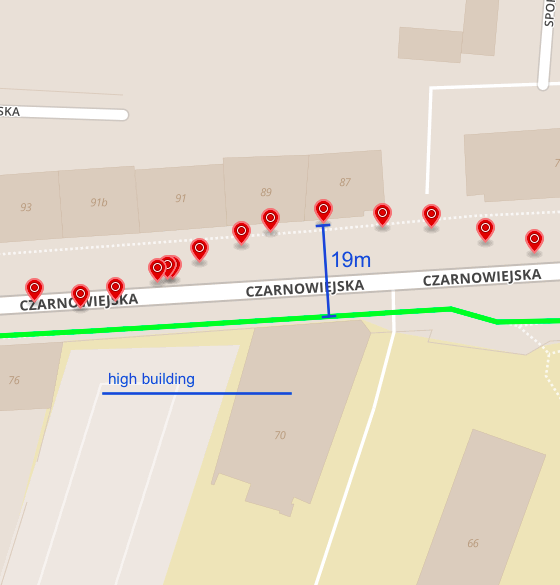
\includegraphics[width=0.9\textwidth]{images/3.png}
    \caption{Green path is the actual path, red pins depict non-filtered readouts. \\ \textit{source: own elaboration}}
    \label{fig:screenexample3}
\end{figure}

\subsection{Example 3: Inaccurate walking readouts} \label{sec:inaccuratereadoutsexample}

Life is not always easy and things like to go badly. As can be seen in the figure \ref{fig:screenexample3}, when approaching high buildings on the south side\footnote{All of the tests were conducted on the north side of the equator.}, readouts became very inaccurate. The readout with largest difference from the actual position was 19 meters, as shown in the figure \ref{fig:screenexample3}. We think this is something that can be solved and we describe proposed solution in the section \ref{sec:futurework}.

\chapter{Conclusions}

\blindtext[1]


\nocite{fy}
\nocite{awb}
\nocite{jtyjycwlnm}
\nocite{rbehs}
\nocite{dp}
\nocite{gapi}
\nocite{hf}
\nocite{gcd}
\nocite{pb}
\nocite{slowpsybx}

% itd.
% \appendix
% \include{dodatekA}
% \include{dodatekB}
% itd.

\printbibliography

\end{document}
